\documentclass[10pt,a4paper]{article}
\usepackage[UTF8,fontset = windows]{ctex}
\setCJKmainfont[BoldFont=黑体,ItalicFont=楷体]{华文中宋}
\usepackage{amssymb,amsmath,amsfonts,amsthm,mathrsfs,dsfont,graphicx}
\usepackage{ifthen,indentfirst,enumerate,color,titletoc}
\usepackage{tikz}
\usepackage{makecell}
\usepackage{longtable}
\usetikzlibrary{arrows,calc,intersections,patterns}
\usepackage[bf,small,indentafter,pagestyles]{titlesec}
\usepackage[top=1in, bottom=1in,left=0.8in,right=0.8in]{geometry}
\renewcommand{\baselinestretch}{1.65}
\newtheorem{defi}{定义~}
\newtheorem{eg}{例~}
\newtheorem{ex}{~}
\newtheorem{rem}{注~}
\newtheorem{thm}{定理~}
\newtheorem{coro}{推论~}
\newtheorem{axiom}{公理~}
\newtheorem{prop}{性质~}
\newcommand{\blank}[1]{\underline{\hbox to #1pt{}}}
\newcommand{\bracket}[1]{(\hbox to #1pt{})}
\newcommand{\onech}[4]{\par\begin{tabular}{p{.9\textwidth}}
A.~#1\\
B.~#2\\
C.~#3\\
D.~#4
\end{tabular}}
\newcommand{\twoch}[4]{\par\begin{tabular}{p{.46\textwidth}p{.46\textwidth}}
A.~#1& B.~#2\\
C.~#3& D.~#4
\end{tabular}}
\newcommand{\vartwoch}[4]{\par\begin{tabular}{p{.46\textwidth}p{.46\textwidth}}
(1)~#1& (2)~#2\\
(3)~#3& (4)~#4
\end{tabular}}
\newcommand{\fourch}[4]{\par\begin{tabular}{p{.23\textwidth}p{.23\textwidth}p{.23\textwidth}p{.23\textwidth}}
A.~#1 &B.~#2& C.~#3& D.~#4
\end{tabular}}
\newcommand{\varfourch}[4]{\par\begin{tabular}{p{.23\textwidth}p{.23\textwidth}p{.23\textwidth}p{.23\textwidth}}
(1)~#1 &(2)~#2& (3)~#3& (4)~#4
\end{tabular}}
\begin{document}
\begin{enumerate}[1.]


%1_21

\item 已知全集$U=\{x|x<2\}$, 集合$A=\{x|x<1\}$, 则$\complement_UA=$\blank{50}.
\item 设集合$A=\{x||x-2|<1, \ x\in\mathbf{R}\}$, $B=\{x|\dfrac{x-3}{x-1}\ge 0\}$, 则$A\cup B=$\blank{50}.
\item 若函数$f(x)=2^x-3$, 则$f^{-1}(1)=$\blank{50}.
\item 设函数$f(x)=\begin{cases} 2^{-x}-1,  & x\le 0,\\ x^\frac 12, & x>0,\end{cases}$ 若$f(x_0)>1$, 则$x_0$的取值范围是\blank{50}.
\item 已知$x\in (0,\dfrac{\pi}2)$, 则方程$\begin{vmatrix} 2\sin x   & 1  \\1  & 2\cos x  \end{vmatrix}=0$的解集是\blank{50}.
\item 关于$x$的不等式$^2+ax+1>0$有解, 则实数$a$的取值范围是\blank{50}.
\item 已知$f(x)=x^2+2(a-2)x+4$, 对$x\in[-3, 1]$, $f(x)>0$恒成立, 则实数$a$的取值范围是\blank{50}.
\item 设正数$a,b$, 当$(a+b)^2+\dfrac{1}{4ab}$取最小值时, $a$的值为\blank{50}.
\item 设椭圆$\Gamma:\dfrac{x^2}{a^2}+{y^2}=1$($a>1$)的左顶点为$A$, 过点$A$的直线$l$与$\Gamma$相交于另一点$B$, 与$y$轴相交于点$C$. 若$|OA|=|OC|$, $|AB|=|BC|$, 则$a=$\blank{50}.
\item 已知常数$b,c\in \mathbf{R}$. 若函数$f(x)=(x^2+x-2)(x^2+bx+c)$为偶函数, 则$b+c=$\blank{50}.
\item 记$a,b,c,d,e,f$为$1,2,3,4,5,6$的任意一个排列, 则使得$(a+b)(c+d)(e+f)$为奇数的排列共有\blank{50}个.
\item 已知函数$f(x)=|x+\dfrac 1x+a|$, 若对任意实数$a$, 关于$x$的不等式$f(x)\ge m$在区间$[\dfrac 12,3]$上总有解, 则实数$m$的取值范围为\blank{50}.
\item 已知$x\in\mathbf{R}$, 则"$x>0$"是"$x>1$"的\bracket{20}.
\fourch{充分非必要条件}{必要非充分条件}{充要条件}{既非充分又非必要条件}
\item 已知$a,b,c$是互不相等的正数, 则下列不等式中正确的是\bracket{20}.
\twoch{$|a-b|<|a-c|+|c-b|$}{$a^2+\dfrac{1}{a^2}\le a+\dfrac{1}{a}$}{$|a-b|+\dfrac{1}{a-b}\ge 2$}{$\sqrt{a+3}-\sqrt{a+1}\le\sqrt{a+2}-\sqrt a$}
\item 设$a,b,c$表示三条互不重合的直线, $\alpha,\beta$表示两个不重合的平面, 则使得``$a\parallel b$''成立	的一个充分条件为\bracket{20}.
\twoch{$a\perp c$, $b\perp c$}{$a\parallel \alpha$, $b\parallel \alpha$}{$a\parallel \alpha$, $a\parallel \beta$, $\alpha \cap \beta =b$}{$b\perp \alpha$, $c\parallel \alpha$, $a\perp c$}
\item 已知函数$y=f(x)$的定义域为$(0,+\infty)$, 满足对任意$x\in (0,+\infty)$, 恒有$f[f(x)-\dfrac 1x]=4$. 若函数$y=f(x)-4$的零点个数为有限的$n$($n\in \mathbf{N}^*$)个, 则$n$的最大值为\bracket{20}.
\fourch{$1$}{$2$}{$3$}{$4$}
\item 如图, 在长方体$ABCD-A_1B_1C_1D_1$中, $2AB=BC=AA_1$, 点$M$为棱$C_1D_1$上的动点.
\begin{center}
    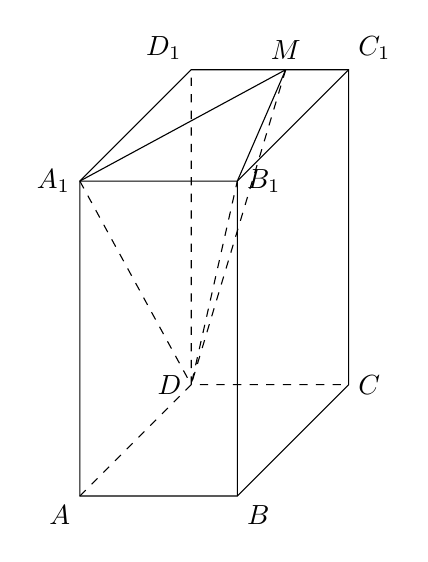
\begin{tikzpicture}
        \draw (0,0) node [below left] {$A$} coordinate (A) --++ (2,0) node [below right] {$B$} coordinate (B) --++ (45:{4/2}) node [right] {$C$} coordinate (C)
        --++ (0,4) node [above right] {$C_1$} coordinate (C1)
        --++ (-2,0) node [above left] {$D_1$} coordinate (D1) --++ (225:{4/2}) node [left] {$A_1$} coordinate (A1) -- cycle;
        \draw (A) ++ (2,4) node [right] {$B_1$} coordinate (B1) -- (B) (B1) --++ (45:{4/2}) (B1) --++ (-2,0);
        \draw [dashed] (A) --++ (45:{4/2}) node [left] {$D$} coordinate (D) --++ (2,0) (D) --++ (0,4);
        \draw ($(D1)!0.6!(C1)$) node [above] {$M$} coordinate (M) (M) -- (A1) (M) -- (B1);
        \draw [dashed] (M) -- (D) -- (B1) (A1) -- (D);
    \end{tikzpicture}
\end{center}
(1) 求三棱锥$D-A_1B_1M$与长方体$ABCD-A_1B_1C_1D_1$的体积比;\\
(2) 若$M$为棱$C_1D_1$的中点, 求直线$DB_1$与平面$DA_1M$所成角的大小.
\item 已知常数$a\in \mathbf{R}^+$, 函数$f(x)=3^x+a^2\cdot 3^{-x}$.\\
(1) 若$a=\sqrt 3$, 解关于$x$的不等式$f(x)<4$;\\
(2) 若$f(x)$在$[3,+\infty)$上为增函数, 求$a$的取值范围.
\item 某居民小区为缓解业主停车难的问题, 拟对小区内一块扇形空地$AOB$进行改建. 如图所示, 平行四边形$OMPN$区域为停车场, 其余部分建成绿地, 点$P$在围墙$\overset\frown{AB}$上, 点$M$和$N$分别在道路$OA$和道路$OB$上, 且$OA=60\text{m}$, $\angle AOB=\dfrac\pi 3$. 设$\angle POB=\theta$.
\begin{center}
    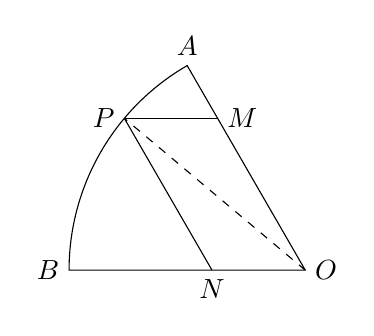
\begin{tikzpicture}
        \draw (0,0) node [left] {$B$} arc (180:140:3) node [left] {$P$} coordinate (P) arc (140:120:3) node [above] {$A$} -- (3,0) node [right] {$O$}-- cycle;
        \draw [dashed] (3,0) -- (P);
        \draw (P) --++ ({3/sin(60)*sin(20)},0) node [right] {$M$};
        \draw (P) --++ (-60:{3/sin(60)*sin(40)}) node [below] {$N$};
    \end{tikzpicture}
\end{center}
(1) 求停车场面积$S$(单位: $\text{m}^2$)关于$\theta$的函数关系式, 并写出$\theta$的取值范围;\\
(2) 求停车场面积$S$的最大值以及相应$\theta$的值.
\item 在平面直角坐标系$xOy$中, 抛物线$\Gamma:y^2=4x$, 点$C(1,0)$. $A,B$为$\Gamma$上的两点, $A$在第一象限, 满足$\overrightarrow{OA}\cdot \overrightarrow{OB}=-4$.\\
(1) 求证: 直线$AB$过定点, 并求定点坐标;\\
(2) 设$P$为$\Gamma$上的动点, 求$\dfrac{|OP|}{|CP|}$的取值范围;\\
(3) 记$\triangle AOB$的面积为$S_1$, $\triangle BOC$的面积为$S_2$, 求$S_1+S_2$的最小值.
\item 已知函数$f(x)=x|x-a|$, 其中$a$为常数.\\
(1) 当$a=1$时, 解不等式$f(x)<2$;\\
(2) 已知$g(x)$是以$2$为周期的偶函数, 且当$0\le x\le 1$时, 有$g(x)=f(x)$. 若$a<0$, 且$g(\dfrac 32)=\dfrac 54$, 求函数$y=g(x)$($x\in [1,2]$)的反函数;\\
(3) 若在$[0,2]$上存在$n$个不同的点$x_i$($i=1,2,\cdots,n$, $n\ge 3$), $x_1<x_2<\cdots <x_n$, 使得$|f(x_1)-f(x_2)|+|f(x_2)-f(x_3)|+\cdots+|f(x_{n-1})-f(x_n)|=8$, 求实数$a$的取值范围.

%2_14

\item 设集合$A=\{1,2,3\}$, $B=\{x|x<3\}$, 则$A\cap B=$\blank{50}.
\item 已知常数$a\in \mathbf{R}$, 函数$f(x)=x^2$($-1\le x\le a$)是偶函数, 则$a=$\blank{50}.
\item 设函数$f(x)=\lg (x+1)$的反函数为$f^{-1}(x)$, 则$f^{-1}(1)=$\blank{50}.
\item 函数$f(x)=\sqrt{\dfrac{1-x}x}$的定义域为\blank{50}.
\item 已知常数$a\in \mathbf{R}$, 设$p:1\le x<2$, $q:x<a$. 若$p$是$q$的充分条件, 则$a$的取值范围为\blank{50}.
\item 关于$x$的方程$\log_2 x+\log_2(x-3)=2$的解为\blank{50}.
\item 已知函数$f(x)$的定义域为$\mathbf{R}$, 满足对任意$x\in \mathbf{R}$, 恒有$f(x)+f(x+2)=4$. 若$f(1)+f(2)=1$, 则$f(2021)-f(2020)=$\blank{50}.
\item 已知常数$a\in \mathbf{R}$, 函数$f(x)=a\cdot 4^x+2^x+1$在$[3,+\infty)$上单调递减, 则$a$的取值范围为\blank{50}.
\item 已知常数$m,n\in \mathbf{Z}$, 若对任意$x\in [0,+\infty)$, 不等式$(mx-2)(x^2-2n)\ge 0$恒成立, 则$m+n$的取值集合为\blank{50}.
\item 已知常数$a\in \mathbf{R}$, 函数$f(x)=x^2-4x+a$, $g(x)=ax^2-8x+4$. 若存在$x_0\in (0,+\infty)$, 使得$f(x_0)$与$g(x_0)$都不是正数, 则$a$的取值范围为\blank{50}.
\item 对任意的非零实数$a,b$, 下列不等式恒成立的是\bracket{20}.
\twoch{$\dfrac ba+\dfrac ab\ge 2$}{$(a+b)(\dfrac 1a+\dfrac 1b)\ge 4$}{$\dfrac{|a+b|}2\ge 2\sqrt{|ab|}$}{$\dfrac{a^2+b^2}{2}\ge (\dfrac{a+b}2)^2$}
\item 设函数$f(x)$的定义域为$\mathbf{R}$, $f(x)$满足对任意$x_1,x_2\in \mathbf{R}$, 当$x_1\ne x_2$时, 恒有$|f(x_1)-f(x_2)|>2|x_1-x_2|$. 对于命题: \textcircled{1} $f(x)$的解析式可以是$f(x)=x^3+2021x$; \textcircled{2} $f(x)$的解析式可以是$f(x)=2021^{-x}$, 下列判断正确的是\bracket{20}.
\twoch{\textcircled{1}、\textcircled{2}均为真命题}{\textcircled{1}、\textcircled{2}均为假命题}{\textcircled{1}为真命题、\textcircled{2}为假命题}{\textcircled{1}为假命题、\textcircled{2}为真命题}
\item 已知常数$a\in \mathbf{R}$, 函数$f(x)=ax^2+\lg \dfrac{1+x}{1-x}$.\\
(1) 若$a=0$, 判断$f(x)$的单调性并证明;\\
(2) 问: 是否存在$a$, 使得$f(x)$为奇函数? 若存在, 求出所有$a$的值; 若不存在, 说明理由.
\item 设函数$f(x)$的定义域为$(0,+\infty)$, 若对任意$x\in (0,+\infty)$, 恒有$f(2x)=2f(x)$, 则称$f(x)$为``$2$阶缩放函数''.\\
(1) 已知函数$f(x)$为``$2$阶缩放函数'', 当$x\in (1,2]$时, $f(x)=1-\log_2 x$, 求$f(2\sqrt{2})$的值;\\
(2) 已知函数$f(x)$为``$2$阶缩放函数'', 当$x\in (1,2]$时, $f(x)=\sqrt{2x-x^2}$, 求证: 函数$y=f(x)-x$在$(1,+\infty)$上无零点.

%3_21
\item 设全集$U=\mathbf{R}$, $A=(-\infty ,3)$, 则$\complement_UA=$\blank{50}.	
\item 函数$f(x)=x^{- \frac 12}$的定义域为\blank{50}.
\item 已知函数$f(x)$的反函数$f^{-1}(x)=\log_2x$, 则$f(-1)=$\blank{50}.
\item 已知球的半径为$2$, 则它的体积为\blank{50}.	
\item 已知$\sin \alpha =-\dfrac{\sqrt 5}5$, $\alpha \in (-\dfrac{\pi}2,\dfrac{\pi}2)$ , 则$\sin (\alpha +\dfrac{3\pi}2)=$\blank{50}.
\item 已知圆锥的底面半径为$1\text{cm}$, 侧面积为$2\pi\text{cm}^2$, 则母线与底面所成角的大小为\blank{50}.
\item 已知$(x^2+\dfrac 2x)^n$的二项展开式中, 所有二项式系数的和为$512$, 则展开式中的常数项为\blank{50}(结果用数值表示).	
\item $f(x)$是偶函数, 当$x\ge 0$时, $f(x)=2^x-1$, 则不等式$f(x)>1$的解集为\blank{50}.
\item 方程$1+\log_2x=\log_2(x^2-3)$的解为\blank{50}.	
\item 已知函数$f(x)=\begin{cases}  x^2+(4a-3)x+3a,& x<0, \\ \log_a(x+1)+1,& x\ge 0, \end{cases}$($a>0$, $a\ne 1$)在$\mathbf{R}$上单调递减, 且关于$x$的方程$|f(x)|=2-x$恰好有两个不相等的实数解, 则$a$的取值范围是\blank{50}.
\item 我国古代数学名著《九章算术》中记载了有关特殊几何体的定义: 阳马指底面为矩形, 一侧棱垂直于底面的四棱锥, 堑堵指底面是直角三角形, 且侧棱垂直于底面的三棱柱. 某堑堵$ABC-A_1B_1C_1$, $AC\perp BC$, 若$A_1A=AB=2$, 当阳马$B-AA_1C_1C$的体积最大时, 二面角$C-A_1B-C_1$的大小为\blank{50}.
\begin{center}
    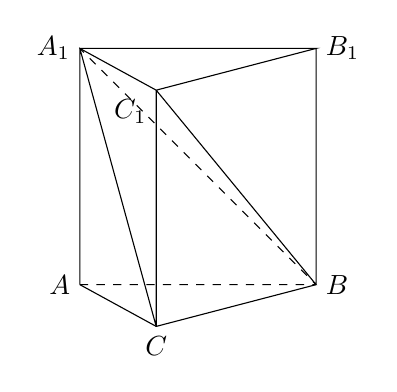
\begin{tikzpicture}[scale = 1.5]
        \draw (-1,0) node [left] {$A$} coordinate (A) -- (225:0.5) node [below] {$C$} coordinate (C) -- (1,0) node [right] {$B$} coordinate (B);
        \draw (A) --++ (0,2) node [left] {$A_1$} coordinate (A1) (B) --++ (0,2) node [right] {$B_1$} coordinate (B1) (C) --++ (0,2) node [below left] {$C_1$} coordinate (C1) (A1) -- (B1) -- (C1) -- (A1) -- (C) (C1) -- (B);
        \draw [dashed] (A) -- (B) -- (A1);
    \end{tikzpicture}
\end{center}
\item 对于全集$\mathbf{R}$的子集$A$, 定义函数$f_A(x)=\begin{cases}
1, &  x\in A,  \\0, & x\in \complement_{\mathbf{R}}A  \end{cases}$为$A$的特征函数, 设$A,B$为全集$\mathbf{R}$的子集,\\
\textcircled{1} 若$A\subseteq B$, 则$f_A(x)\le f_B(x)$; \textcircled{2} $f_{\complement_{\mathbf{R}}A}(x)=1-f_A(x)$;\\
\textcircled{3} ${f_{A\cap B}}(x)=f_A(x)\cdot f_B(x)$; \textcircled{4} $f_{A\cup B}(x)=f_A(x)+f_B(x)$;\\ \textcircled{5} $f_{A\cap \complement_\mathbf{R}B}(x)=f_A(x)-f_B(x)$; \textcircled{6} 对于任意$x\in \mathbf{R}$, 若$f_A(x)\cdot f_B(x)=0$恒成立, 则$A\cap B=\varnothing$.\\
其中正确的命题为\blank{50}(填所有正确命题的序号).
\item 已知实数$a,b$满足$a>b$, 则下列不等式中恒成立的是\bracket{20}。
\fourch{$a^2>b^2$}{$\dfrac 1a<\dfrac 1b$}{$|a|>|b|$}{$2^a>2^b$}
\item 下列函数中, 值域为$(0,+\infty)$的是\bracket{20}.
\fourch{$y=x^2$}{$y=\dfrac 2x$}{$y=2^x$}{$y=|\log_2x|$}
\item 从正方体的$8$个顶点中选取$4$个作为顶点, 可得到四面体的个数为\bracket{20}.
\fourch{$\mathrm{C}_8^4-12$}{$\mathrm{C}_8^4-8$}{$\mathrm{C}_8^4-6$}{$\mathrm{C}_8^4-4$}
\item 设集合$A=\{y|y=a^x,\ x>0\}$(其中常数$a>0,  \ a\ne 1$), $B=\{y|y=x^k,\ x\in A\}$(其中常数$k\in \mathbf{Q}$), 则``$k<0$''是``$A\cap B=\varnothing$''的\bracket{20}.
\twoch{充分非必要条件}{必要非充分条件}{充分必要条件}{既非充分又非必要条件}
\item 如图所示, 在直三棱柱$ABC-A_1B_1C_1$中, 底面是等腰直角三角形, $\angle ACB=90^\circ$, $CA=CB=CC_1=2$. 点$D,D_1$分别是棱$AC,A_1C_1$的中点.
\begin{center}
    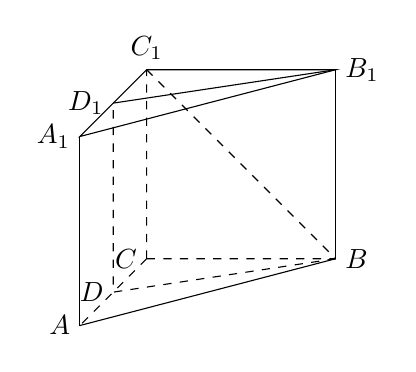
\begin{tikzpicture}[scale = 1.2]
        \draw [dashed] (0,0) node [left] {$C$} coordinate (C) -- (2,0) node [right] {$B$} coordinate (B) (C) -- (0,2) node [above] {$C_1$} coordinate (C1) (C) -- (225:1) node [left] {$A$} coordinate (A);
        \draw (A) --++ (0,2) node [left] {$A_1$} coordinate (A1) (B) --++ (0,2) node [right] {$B_1$} coordinate (B1);
        \draw (A) -- (B) (A1) -- (B1) -- (C1) -- cycle;
        \draw ($(A)!0.5!(C)$) node [left] {$D$} coordinate (D) ++ (0,2) node [left] {$D_1$} coordinate (D1);
        \draw (B1) -- (D1);
        \draw [dashed] (B) -- (D) -- (D1) (C1) -- (B);
    \end{tikzpicture}
\end{center}
(1)	求四棱锥$C-AA_1B_1B$的体积;\\
(2)	求直线$BC_1$与平面$DBB_1D_1$所成角的大小.
\item 设常数$k\in \mathbf{R}$, $f(x)=k\cos^2x+\sqrt 3\sin x\cos x$, $x\in \mathbf{R}$.\\
(1) 若$\tan \alpha =2$且$f(\alpha)=\sqrt 3$, 求实数$k$的值;\\
(2) 设$k=1$, $\triangle ABC$中, 内角$A,B,C$的对边分别为$a,b,c$. 若$f(A)=1$, $a=\sqrt 7$, $b=3$, 求$\triangle ABC$的面积$S$.
\item 东西向的铁路上有两个道口$AB$, 铁路两侧的公路分布如图, $C$位于$A$的南偏西$15^\circ$, 且位于$B$的南偏东$15^\circ$方向, $D$位于$A$的正北方向, $AC=AD=2km$, $C$处一辆救护车欲通过道口前往$D$处的医院送病人, 发现北偏东$45^\circ$方向的$E$处(火车头位置)有一列火车自东向西驶来, 若火车通过每个道口都需要$1$分钟, 救护车和火车的速度均为$60\text{km/h}$.
\begin{center}
    \begin{tikzpicture}[>=latex]
        \draw (-2,0) -- (2,0) (0,0) node [above right] {$A$} -- (0,2) node [right] {$D$};
        \draw (0,0) --++ (-105:2) node [below] {$C$} coordinate (C) --++ (105:2) node [above left] {$B$} -- (0,2); 
        \draw ({sqrt(2)},0) node [above] {$E$} -- (C);
        \draw [->] (-2,1) --++ (0.5,0) node [right] {东};
        \draw [->] (-2,1) --++ (0,0.5) node [above] {北};
    \end{tikzpicture}
\end{center}
(1) 判断救护车通过道口$A$是否会受火车影响, 并说明理由;\\
(2) 为了尽快将病人送到医院, 救护车应选择$AB$中的哪个道口? 通过计算说明.
\item 已知函数$f(x)=\dfrac{ax^2+1}{bx+c}$是奇函数, $a,b,c$为常数.\\
(1)	求实数$c$的值;\\
(2)	若$a,b\in \mathbf{Z}$, 且$f(1)=2$, $f(2)<3$, 求$f(x)$的解析式;\\
(3) 已知$b>0$, 若$f(x)\ge f(1)$在$(0,+\infty)$上恒成立, 且$\{x|f[f(x)]\ge x\}\cap [1,2]\ne \varnothing$, 求$b$的取值范围.
\item 记函数$f(x)$的定义域为$D$. 如果存在实数$a$、$b$使得$f(a-x)+f(a+x)=b$对任意满足$a-x\in D$且$a+x\in D$的$x$恒成立, 则称$f(x)$为$\Psi$函数.\\
(1) 设函数$f(x)=\dfrac 1x-1$, 试判断$f(x)$是否为$\Psi$函数, 若是求出$a,b$, 若不是请说明理由;\\
(2) 设函数$g(x)=\dfrac 1{2^x+t}$, 其中常数$t\ne 0$, 证明: $g(x)$是$\Psi$函数;\\
(3) 若$h(x)$是定义在$\mathbf{R}$上的$\Psi$函数, 且函数$h(x)$的图像关于直线$x=m$($m$为常数)对称, 试判断$h(x)$是否为周期函数? 并证明你的结论.

%4_16
\item 不等式$\dfrac 1x\le 3$的解集是\blank{50}.
\item 若函数$y=\sin (2x+\dfrac{\pi }4)$, 则它的最小正周期$T=$\blank{50}.
\item 若函数$y=\log_2(x-m)+1$的反函数的图像经过点$(1,3)$, 则实数$m=$\blank{50}.
\item 函数$f(x)=x+\dfrac 1{x-2}$的值域是\blank{50}.
\item 已知函数$f(x)$的周期为$2$, 且当$0<x\le 1$时, $f(x)=\log_4x$, 那么$f(\dfrac 92)=$\blank{50}
\item 已知集合$M=\{y|y=3\sin x,x\in \mathbf{R}\}$, $N=\{x||x|<a\}$, 若$M\subseteq N$, 则实数$a$的取值范围是\blank{50}.
\item 函数$f(x)=|x^2-1|+|x-2|$的最小值是\blank{50}.
\item 已知函数$f(x)=\begin{cases}  -x^2-2x, & x\le a,  \\-x+2, &x>a,  \end{cases}$ 若存在实数$x_0$, 使得对于任意的实数$x$都有$f(x)\le f(x_0)$成立, 则实数$a$的取值范围是\blank{50}.
\item 函数$f(x)=\dfrac x{x+1}+\dfrac{x+1}{x+2}+\dfrac{x+2}{x+3}$图像的对称中心的坐标是\blank{50}.
\item 若$f(x)=|x+1|+|x+2|+\cdots +|x+2020|+|x-1|+|x-2|+\cdots +|x-2020|$, $x\in \mathbf{R}$, 且$f(a^2-3a+2)=f(a-1)$, 则满足条件的所有整数$a$的和是\blank{50}.
\item 王昌龄《从军行》中两句诗``黄沙百战穿金甲, 不破楼兰终不还'', 其中后一句中``攻破楼兰''是``返回家乡''的\bracket{20}条件.
\fourch{充分}{必要}{充要}{既不充分也不必要}
\item 为了得到函数$y=\sin (2x+\dfrac{\pi}3)$的图像, 可将函数$y=\sin x$的图像\bracket{20}.
\fourch{左移$\dfrac{\pi}3$个长度}{右移$\dfrac{\pi}3$个长度}{左移$\dfrac{\pi}6$个长度}{右移$\dfrac{\pi}6$个长度}
\item 已知$M$、$N$、$P\subseteq \mathbf{R}$, $M=\{x|f(x)=0\}$, $N=\{x|g(x)=0\}$, $P=\{x|f(x)g(x)=0\}$, 则集合$P$恒满足的关系为\bracket{20}.
\fourch{$P=M\cup N$}{$P\ne \varnothing$}{$P=\varnothing$}{$P\subseteq (M\cup N)$}
\item 已知$a_1$、$a_2$与$b_1$、$b_2$是$4$个不同的实数, 关于x的方程$|x-a_1|+|x-a_2|=|x-b_1|+|x-b_2|$的解集为$A$, 则集合$A$中元素的个数为\bracket{20}.
\twoch{$1$个}{$0$个或$1$个或$2$个}{$0$个或$1$个或$2$个或无限个}{$1$个或无限个}
\item 设函数$f(x)$是定义在$[a,b]$上的函数, 若存在$x_0\in (a,b)$, 使得$f(x)$在$[a,x_0]$上单调递增, 在$[x_0,b]$上单调递减, 则称$f(x)$为$[a,b]$上的单峰函数, $x_0$称为峰点.\\
(1) 判断下列函数中, 哪些是$[0,2]$上的单峰函数? 若是, 指出峰点; 若不是, 说出原因;\\
\textcircled{1}  $f_1(x)=3x-x^2$; \textcircled{2}  $f_2(x)=\dfrac{2x}{{x^2}+1}$;\\
(2) 若函数$f(x)$是区间$[0,1]$上的单峰函数, 证明: 对任意的$x_1$、$x_2\in (0,1)$, $x_1<x_2$, 若$f(x_1)\ge f(x_2)$, 则峰点在区间$(0,x_2)$内; 若$f(x_1)\le f(x_2)$, 则峰点在区间$(x_1,1)$内.
\item 设$\mu (x)$表示不小于$x$的最小整数, 例如$\mu(0.3)=1$, $\mu(-2.5)=2$.\\
(1) 解方程$\mu(x-1)=3$;\\
(2) 设$f(x)=\mu (x\cdot \mu (x))$, $n\in \mathbf{N}^*$, 试分别求出$f(x)$在区间$(0,1]$、$(1,2]$以及$(2,3]$上的值域; 若$f(x)$在区间$(0,n]$上的值域为$M_n$, 求集合$M_n$中的元素的个数;\\
(3) 设实数$a>0$, $g(x)=x+a\cdot \dfrac{\mu (x)}x-2$, $h(x)=\dfrac{\sin (\pi x)+2}{x^2-5x+7}$, 若对于任意$x_1,x_2\in (2,4]$都有$g(x_1)>h(x_2)$, 求实数$a$的取值范围.

%5_21
\item 函数$y=\log_2(4-x^2)$的定义域是\blank{50}.
\item 如图所示, 弧长为$\dfrac{\pi}2$, 半径为$1$的扇形(及其内部)绕$OB$
所在的直线旋转一周, 所形成的几何体的表面积为\blank{50}.
\begin{center}
    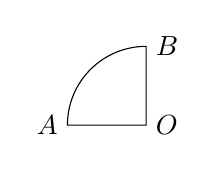
\begin{tikzpicture}
        \draw (0,0) node [right] {$O$} -- (-1,0) node [left] {$A$} arc (180:90:1) node [right] {$B$} -- cycle;
    \end{tikzpicture}
\end{center}
\item 函数$f(x)=1-3\sin ^2(x+\dfrac{\pi}4)$的最小正周期为\blank{50}.
\item 从$5$名志愿者中选出$3$名, 分别从事布置、迎宾、策划三项不同的工作, 每人承担一项工作, 则不同的选派方案有\blank{50}种(用数值作答).
\item 已知函数$f(x)=a\cdot 2^x+3-a$($a\in \mathbf{R}$且$a\ne 0$)的反函数为$y=f^{-1}(x)$, 则函数$y=f^{-1}(x)$的图像经过的定点的坐标为\blank{50}.
\item 在$(x-a)^{10}$的展开式中, $x^7$的系数是$15$, 则实数$a=$\blank{50}.
\item 已知$\cos (\dfrac{\pi}4+\alpha)=\dfrac 13$, 则$\cos (\dfrac{\pi}2-2\alpha)=$\blank{50}.
\item 集合$\{x|\cos(\pi \cos x)=0,\ x\in [0,\pi]\}=$\blank{50}(用列举法表示).
\item 在$\triangle ABC$中, 角$A,B,C$的对边分别为$a,b,c$, 面积为$S$, 且$4S=(a+b)^2-c^2$, 则$\cos C=$\blank{50}.
\item 如图, 在三棱锥$D-AEF$中, $A_1,B_1,C_1$分别是$DA,DE,DF$的中点, $B,C$分别是$AE,AF$的中点, 设三棱柱$ABC-A_1B_1C_1$的体积为$V_1$, 三棱锥$D-AEF$的体积为$V_2$, 则$V_1:V_2=$\blank{50}.
\begin{center}
    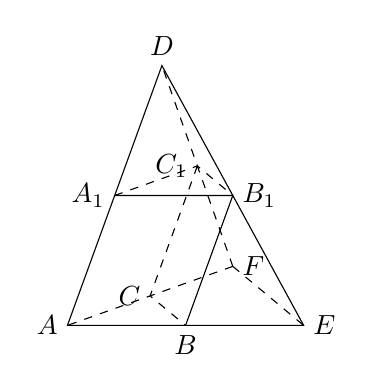
\begin{tikzpicture}[scale = 1.5]
        \draw (0,0) node [left] {$A$} coordinate (A) -- (2,0) node [right] {$E$} coordinate (E) -- (0.8,2.2) node [above] {$D$} coordinate (D) -- cycle;
        \draw [dashed] (1.4,0.5) node [right] {$F$} coordinate (F) -- (A) (F) -- (D) (F) -- (E);
        \draw ($(A)!0.5!(E)$) node [below] {$B$} coordinate (B) -- ($(D)!0.5!(E)$) node [right] {$B_1$} coordinate (B1) -- ($(A)!0.5!(D)$) node [left] {$A_1$} coordinate (A1);
        \draw [dashed] ($(D)!0.5!(F)$) node [left] {$C_1$} coordinate (C1) -- ($(A)!0.5!(F)$) node [left] {$C$} coordinate (C) -- (B) (A1) -- (C1) -- (B1);
    \end{tikzpicture}
\end{center}
\item 集合$A=\{y|y=\log_{\frac 12}x-x,1\le x\le 2\}$, $B=\{x|x^2-5tx+1\le 0\}$, 若$A\cap B=A$, 则实数$t$的取值范围是\blank{50}.
\item 若定义在实数集$\mathbf{R}$上的奇函数$y=f(x)$的图像关于直线$x=1$对称, 且当$0\le x\le 1$时, $f(x)=x^{\frac 13}$, 则方程$f(x)=\dfrac 13$在区间$(-4,10)$内的所有实根之和为\blank{50}.
\item 若空间中三条不同的直线$l_1$、$l_2$、$l_3$, 满足$l_1\perp l_2$, $l_2\parallel l_3$, 则下列结论一定正确的是\bracket{20}.
\twoch{$l_1\perp l_3$}{$l_1\parallel l_3$}{$l_1$、$l_3$既不平行也不垂直}{$l_1$、$l_3$相交且垂直}
\item 若$a>b>0$, $c<d<0$, 则一定有\bracket{20}.
\fourch{$ad>bc$}{$ad<bc$}{$ac<bd$}{$ac>bd$}
\item 函数$f(x)=|x^2-a|$在区间$[-1,1]$上的最大值是$a$, 那么实数$a$的取值范围是\bracket{20}.
\fourch{$[0,+\infty)$}{$[\dfrac 12,1]$}{$[\dfrac 12,+\infty)$}{$[1,+\infty)$}
\item 已知函数$f(x)=\begin{cases}\log_{\frac 12}(1-x), & -1\le x\le n,  \\ 2^{2-|x-1|}-3, & n<x\le m,  \end{cases}$($n<m$)的值域是$[-1,1]$, 有下列结论:
\textcircled{1} 当$n=0$时, $m$的取值范围为$(0,2]$; \textcircled{2}  当$n=\dfrac 12$时, $m$的取值范围为$(\dfrac 12,2]$; \textcircled{3}  当$n\in [0,\dfrac 12)$时, $m$的取值范围为$[1,2]$; \textcircled{4}  当$n\in [0,\dfrac 12)$时, $m$的取值范围为$(n,2]$;
其中结论正确的所有的序号是\bracket{20}.
\fourch{\textcircled{1}\textcircled{2}}{\textcircled{3}\textcircled{4}}{\textcircled{2}\textcircled{3}}{\textcircled{2}\textcircled{4}}
\item 如图, 在正三棱柱$ABC-A_1B_1C_1$中, $AA_1=4$, 异面直线$BC_1$与$AA_1$所成角的大小为$\dfrac{\pi}3$.
\begin{center}
    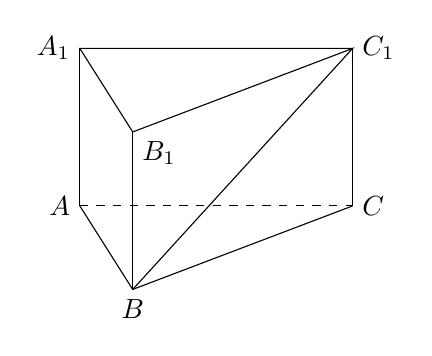
\begin{tikzpicture}[scale = 1]
        \draw ({-sqrt(3)},0) node [left] {$A$} coordinate (A) -- (225:1.5) node [below] {$B$} coordinate (B) -- ({sqrt(3)},0) node [right] {$C$} coordinate (C);
        \draw (A) --++ (0,2) node [left] {$A_1$} coordinate (A1) (B) --++ (0,2) node [below right] {$B_1$} coordinate (B1) (C) --++ (0,2) node [right] {$C_1$} coordinate (C1);
        \draw (B) -- (C1) -- (B1) -- (A1) -- (C1);
        \draw [dashed] (A) -- (C);
    \end{tikzpicture}
\end{center}
(1) 求正三棱柱$ABC-A_1B_1C_1$的体积;\\
(2) 求直线$BC_1$与平面$AA_1C_1C$所成角的大小.
\item 已知函数$f(x)=\dfrac 32\sin \omega x+\dfrac{\sqrt 3}2\cos \omega x$(其中$\omega >0$).\\
(1)	若$\omega =2$, $0<\alpha <\pi$, 且$f(\alpha)=\dfrac 32$, 求$\alpha$的值;\\
(2)	若函数$f(x)$的最小正周期为$3\pi$, 求$\omega$的值, 并求函数$f(x)$在$[0,\pi]$上的单调递增区间.
\item 如图, 有一块边长为$1$的正方形区域$ABCD$, 在点$A$处有一个可转动的探照灯, 其照射角$\angle PAQ$始终为$45^\circ$(其中点$P$、$Q$分别在边$BC$、$CD$上), 设$\angle PAB=\theta$, $\tan \theta =t$.
\begin{center}
    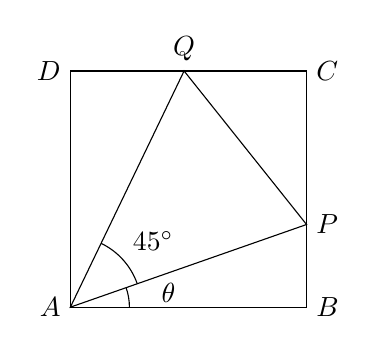
\begin{tikzpicture}[scale = 1.5]
        \draw (0,0) node [left] {$A$} coordinate (A) -- (2,0) node [right] {$B$} coordinate (B) -- (2,2) node [right] {$C$} coordinate (C) -- (0,2) node [left] {$D$} coordinate (D) -- cycle;
        \draw (2,0.7) node [right] {$P$} coordinate (P) -- ({26/27},2) node [above] {$Q$} coordinate (Q) -- (A) -- cycle;
        \draw (0.5,0) arc (0:atan(0.35):0.5);
        \draw ({atan(0.35)/2}:0.7) node [right] {$\theta$};
        \draw ({atan(0.35)}:0.6) arc ({atan(0.35)}:{atan(0.35)+45}:0.6);
        \draw ({atan(0.35)+22.5}:0.6) node [above right] {$45^\circ$};
    \end{tikzpicture}
\end{center}
(1) 当三点$C$、$P$、$Q$不共线时, 求直角$\triangle CPQ$的周长;\\
(2) 设探照灯照射在正方形$ABCD$内部区域$PAQC$的面积为$S$, 试求$S$的最大值.
\item 定义区间$(m,n)$、$[m,n]$、$(m,n]$、$[m,n)$的长度均为$n-m$, 已知不等式$\dfrac 7{6-x}\ge 1$的解集为$A$.\\
(1) 求$A$的长度;\\
(2) 函数$f(x)=\dfrac{(a^2+a)x-1}{a^2x}$($a\in \mathbf{R}$, $a\ne 0$)的定义域与值域都是$[m,n]$($n>m$), 求区间$[m,n]$的最大长度;\\
(3) 关于$x$的不等式$\log_2x+\log_2(tx+3t)<2$的解集为$B$, 若$A\cap B$的长度为$6$, 求实数$t$的取值范围.
\item 对于函数$y=f(x)$($x\in D$), 如果存在实数$a$、$b$($a\ne 0$, 且$a=1$, $b=0$不同时成立), 使得$f(x)=f(ax+b)$对$x\in D$恒成立, 则称函数$f(x)$为``$(a,b)$映像函数''.\\
(1) 判断函数$f(x)=x^2-2$是否是``$(a,b)$映像函数'', 如果是, 请求出相应的$a$、$b$的值, 若不是, 请说明理由;\\
(2) 已知函数$y=f(x)$是定义在$[0,+\infty)$上的``$(2,1)$映像函数'', 且当$x\in [0,1)$时, $f(x)=2^x$, 求函数$y=f(x)$($x\in [3,7)$)的反函数;\\
(3) 在(2)的条件下, 试构造一个数列$\{a_n\}$, 使得当$x\in [a_n,{a_{n+1}})$($n\in \mathbf{N}^*$)时, $2x+1$的取值范围为$[{a_{n+1}},{a_{n+2}})$, 并求$x\in [a_n,{a_{n+1}})$($n\in \mathbf{N}^*$)时, 函数$y=f(x)$的解析式, 及$y=f(x)$($x\in [0,+\infty)$)的值域.

%6_21

\begin{center}
    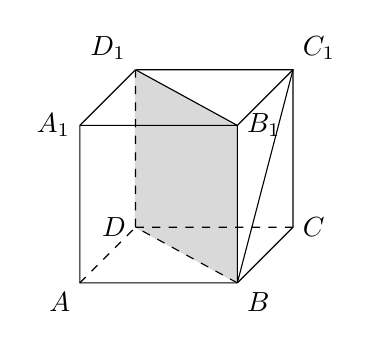
\begin{tikzpicture}
        \draw (0,0) node [below left] {$A$} coordinate (A) --++ (2,0) node [below right] {$B$} coordinate (B) --++ (45:{2/2}) node [right] {$C$} coordinate (C)
        --++ (0,2) node [above right] {$C_1$} coordinate (C1)
        --++ (-2,0) node [above left] {$D_1$} coordinate (D1) --++ (225:{2/2}) node [left] {$A_1$} coordinate (A1) -- cycle;
        \draw (A) ++ (2,2) node [right] {$B_1$} coordinate (B1) --++ (45:{2/2}) (B1) ++ (-2,0);
        \draw [dashed] (A) --++ (45:{2/2}) node [left] {$D$} coordinate (D) ++ (2,0) (D) ++ (0,2);
        \filldraw [gray!30] (B) -- (D) -- (D1) -- (B1) -- cycle;
        \draw (B) --  (C1) (D1) -- (B1) -- (B) (B1) -- (A1);
        \draw [dashed] (B) -- (D) -- (D1) (D) -- (C);
    \end{tikzpicture}
\end{center}

\begin{center}
    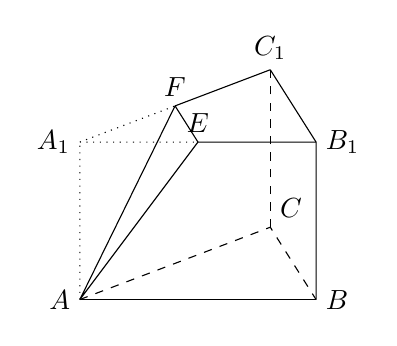
\begin{tikzpicture}
        \draw (0,0) node [left] {$A$} coordinate (A) -- (3,0) node [right] {$B$} coordinate (B) (A) ++ (1.5,0) ++ (45:{sqrt(3)*3/4}) node [above right] {$C$} coordinate (C);
        \draw (A) ++ (0,2) node [left] {$A_1$} coordinate (A1);
        \draw (B) ++ (0,2) node [right] {$B_1$} coordinate (B1);
        \draw [dashed] (C) --++ (0,2) node [above] {$C_1$} coordinate (C1);
        \draw (B) -- (B1) -- (C1);
        \draw [dashed] (A) -- (C) -- (B);
        \draw ($(A1)!0.5!(B1)$) node [above] {$E$} coordinate (E) ($(A1)!0.5!(C1)$) node [above] {$F$} coordinate (F);
        \draw [dotted] (A1) -- (F) (A1) -- (E) (A) -- (A1);
        \draw (A) -- (E) -- (B1) (E) -- (F) (A) -- (F) -- (C1);
    \end{tikzpicture}
\end{center}

\begin{center}
    \begin{tikzpicture}[>=latex]
        \draw [->] (-1,0) -- (3,0) node [below] {$x$};
        \draw [->] (0,-2.5) -- (0,2.5) node [left] {$y$};
        \draw (0,0) node [below left] {$O$};
        \draw [domain = -45:135, samples = 200] plot ({\x/180*pi},{2*sin(2*\x+90)});
        \filldraw ({-pi/4},0) circle (0.03) node [above left] {$-\frac\pi 4$} ({pi/4},0) circle (0.03) node [above right] {$\frac\pi 4$};
        \draw (0,2) node [above left] {$2$};
        \draw [dashed] (0,-2) node [left] {$-2$} -- ({pi/2},-2) -- ({pi/2},0);
    \end{tikzpicture}
\end{center}
%7_21

\item 计算$\displaystyle \lim_{n\to\infty}\dfrac{4n+4}{5n+1}=$.
\item 设全集$U=\mathbf{R}$集合$A=\{-2,-1,0,1,2\}$, $B=\{x|x\ge 0\}$, 则$A\cap \complement_UB=$\blank{50}.
\item 不等式$\dfrac 1{x-1}\ >1$的解集为\blank{50}.
\item 若一个球的体积为$36\pi$, 则它的表面积为\blank{50}.
\item 设复数$z$满足$z+2\overline z=3-\mathrm{i}$($\mathrm{i}$为虚数单位), 则$z=$\blank{50}.
\item 数列$\{a_n\}$的通项公式是$a_n=(\dfrac 23)^n$, $n\in \mathbf{N}^*$, 则数列$\{a_n\}$所有项的和为\blank{50}.
\item 某班级要从$5$名男生和$3$名女生中选出$3$人参加公益活动, 则在选出的$3$人中男、女生均有的概率为\blank{50}(结果用最简分数表示).
\item 已知$\omega,t>0$, 函数$f(x)=\begin{vmatrix}
\sqrt 3 & \sin \omega x  \\ 1  & \cos \omega x  \end{vmatrix}$的最小正周期为$2\pi$, 将$f(x)$的图像向左平移$t$个单位, 所得图像对应的函数为偶函数, 则$t$的最小值为\blank{50}.
\item 设函数$f(x)=\begin{cases} x^6, &  x\ge 1,  \\ -2x-1, &  x\le -1,  \end{cases}$ 则当$x\le -1$时, 则$f[f(x)]$表达式的展开式中含$x^2$项的系数是\blank{50}.
\item 已知数列$\{a_n\}$满足$S_n=\dfrac32a_n+n$(其中$S_n$为数列$\{a_n\}$前$n$项和), 则数列$\{a_n\}$的通项公式是\blank{50}.
\item 如图, 已知半圆$O$的直径$AB=4$, $\triangle OAC$是等边三角形, 若点$P$是边$AC$(包含端点$A,C$)上的动点, 点$Q$在弧$\overset\frown{BC}$上, 且满足$OQ\perp OP$, 则$\overrightarrow{OP}\cdot \overrightarrow{BQ}$的最小值为\blank{50}.
\begin{center}
    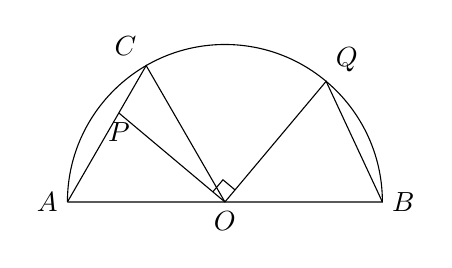
\begin{tikzpicture}
        \draw (-2,0) node [left] {$A$} coordinate (A) arc (180:0:2) node [right] {$B$} coordinate (B) -- (A);
        \draw (0,0) node [below] {$O$} coordinate (O) --++ (120:2) node [above left] {$C$} coordinate (C) -- (A);
        \draw (O) --++ (50:2) node [above right] {$Q$} coordinate (Q) -- (B);
        \path [name path = AC] (A) -- (C);
        \path [name path = OP] (O) -- (140:2);
        \path [name intersections = {of = AC and OP, by = P}];
        \draw (O) -- (P) node [below] {$P$};
        \draw (50:0.2) --++ (140:0.2) --++ (230:0.2);
    \end{tikzpicture}
\end{center}
\item 如果一个数列由有限个连续的正整数组成(数列的项数大于$2$), 且所有项之和为$N$, 那么称该数列为$N$型标准数列, 例如, 数列$2, 3, 4, 5, 6$为$20$型标准数列, 则$2668$型标准数列的个数为\blank{50}.
\item 设$\alpha \beta$为两个不同平面, 已知直线$l$在平面$\alpha$内, 则``$\alpha \perp \beta$''是``$l\perp \beta$''
的\bracket{20}.
\fourch{充分不必要条件}{必要不充分条件}{充要条件}{既不充分也不必要条件}
\item 某中学的高一、高二、高三共有学生$1350$人, 其中高一$500$人, 高三比高二少$50$人, 为了解该校学生健康状况, 现采用分层抽样方法进行调查, 在抽取的样本中有高一学生$120$人, 则该样本中的高二学生人数为\bracket{20}.
\fourch{$80$}{$96$}{$108$}{$110$}
\item 已知$\overrightarrow{a}$、$\overrightarrow b$均为单位向量, 且$\overrightarrow a\cdot\overrightarrow b=0$. 若$|\overrightarrow c-4\overrightarrow a |+| \overrightarrow c-3\overrightarrow b |=5$, 则$| \overrightarrow c+\overrightarrow a|$的取值范围是\bracket{20}.
\fourch{$[3,\sqrt{10}]$}{$[3,5]$}{$[3,4]$}{$[ \sqrt{10},5]$}
\item 正四面体$ABCD$的体积为$1$, $O$为其中心, 正四面体$EFGH$与正四面体$ABCD$关于点$O$对称, 则这两个正四面体的公共部分的体积为\bracket{20}.
\item \begin{center}
    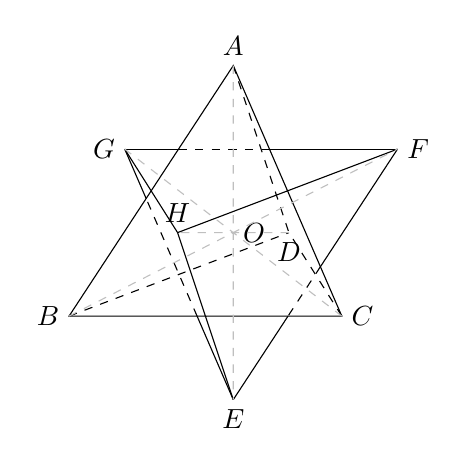
\begin{tikzpicture}[scale = 2]
        \draw ({-sqrt(3)/2-sqrt(2)/8},{-sqrt(2)/8})  node [left] {$B$} coordinate (B)  ({sqrt(3)/2-sqrt(2)/8},{-sqrt(2)/8}) node [right] {$C$} coordinate (C)  ({sqrt(2)/4},{sqrt(2)/4}) node [below] {$D$} coordinate (D) (C)  (0,{sqrt(2)}) node [above] {$A$} coordinate (A);
        \draw (0,{sqrt(2)/4}) node [right] {$O$} coordinate (O);
        \draw ($(A)!2!(O)$) node [below] {$E$} coordinate (A1) ($(B)!2!(O)$) node [right] {$F$} coordinate (B1) ($(C)!2!(O)$) node [left] {$G$} coordinate (C1) ($(D)!2!(O)$) node [above] {$H$} coordinate (D1);
        \draw (A) -- (B) -- (C) -- cycle (D1) -- (A1) (D1) -- (B1) (D1) -- (C1);
        \draw [dashed] (A) -- (D) (B) -- (D) (C) -- (D);
        \path [name path = B1C1] (B1) -- (C1);
        \path [name path = C1A1] (C1) -- (A1);
        \path [name path = A1B1] (A1) -- (B1);
        \path [name path = AB] (A) -- (B);
        \path [name path = BC] (B) -- (C);
        \path [name path = CA] (C) -- (A);
        \path [name intersections = {of = B1C1 and AB, by = U}];
        \path [name intersections = {of = B1C1 and CA, by = V}];
        \draw (C1) -- (U) (V) --(B1);
        \draw [dashed] (U) -- (V);
        \path [name intersections = {of = A1B1 and CA, by = S}];
        \path [name intersections = {of = A1B1 and BC, by = T}];
        \draw (B1) -- (S) (T) --(A1);
        \draw [dashed] (S) -- (T);
        \path [name intersections = {of = C1A1 and BC, by = X}];
        \path [name intersections = {of = C1A1 and AB, by = Y}];
        \draw (A1) -- (X) (Y) --(C1);
        \draw [dashed] (X) -- (Y);
        \draw [dashed,gray!50] (A) -- (A1) (B) -- (B1) (C) -- (C1) (D) -- (D1);
    \end{tikzpicture}
\end{center}
\fourch{$\dfrac13$}{$\dfrac12$}{$\dfrac23$}{$\dfrac34$}
\item 如图, 已知正三棱柱$ABC-A_1B_1C_1$的底面积为$\dfrac{9\sqrt 3}4$, 侧面积为$36$.\\
\begin{center}
    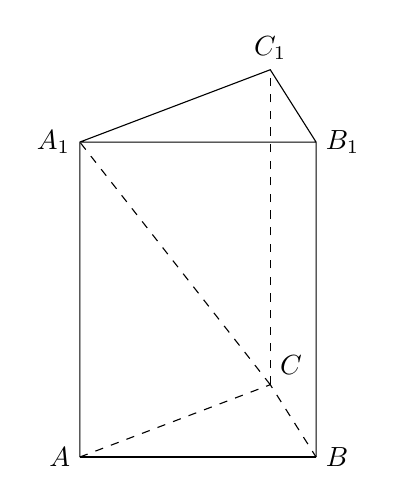
\begin{tikzpicture}
        \draw (0,0) node [left] {$A$} coordinate (A) -- (3,0) node [right] {$B$} coordinate (B) (A) ++ (1.5,0) ++ (45:{sqrt(3)*3/4}) node [above right] {$C$} coordinate (C);
        \draw (A) ++ (0,4) node [left] {$A_1$} coordinate (A1);
        \draw (B) ++ (0,4) node [right] {$B_1$} coordinate (B1);
        \draw [dashed] (C) --++ (0,4) node [above] {$C_1$} coordinate (C1);
        \draw (B) -- (B1) -- (C1) -- (A1) -- (A) (A1) --(B1);
        \draw [dashed] (A) -- (C) -- (B) (C) -- (A1);
    \end{tikzpicture}
\end{center}
(1) 求正三棱柱$ABC-A_1B_1C_1$的体积;\\
(2) 求异面直线$A_1C$与$AB$所成的角的大小;
\item 已知$\triangle ABC$的面积为$S$, 且$\overrightarrow{AB}\cdot \overrightarrow{AC}=S$.\\
(1)	求$\sin A,\cos A,\tan 2A$的值;\\
(2)	若$B=\dfrac{\pi }4$, $|\overrightarrow{CA}-\overrightarrow{CB}|=6$, 求$\triangle ABC$的面积$S$.
\item 某温室大棚规定: 一天中, 从中午$12$点到第二天上午$8$点为保温时段, 其余$4$小时为工人作业时段. 从中午$12$点连续测量$20$小时, 得出此温室大棚的温度$y$(单位: 度)与时间$t$(单位: 小时, $t\in [0,20]$)近似地满足函数$y=|t-13|+\dfrac b{t+2}$关系, 其中, $b$为大棚内一天中保温时段的通风量.\\
(1) 若一天中保温时段的通风量保持$100$个单位不变, 求大棚一天中保温时段的最低温度(精确到$0.1^\circ\text{C}$);\\
(2) 若要保持大棚一天中保温时段的最低温度不小于$17^\circ\text{C}$, 求大棚一天中保温时段通风量的最小值.
\item 已知直线$l:x=t$($0<t<2$)与椭圆$\Gamma:\dfrac{x^2}4+\dfrac{y^2}2=1$相交于$A$, $B$两点, 其中$A$在第一象限, $M$是椭圆上一点.
\begin{center}
    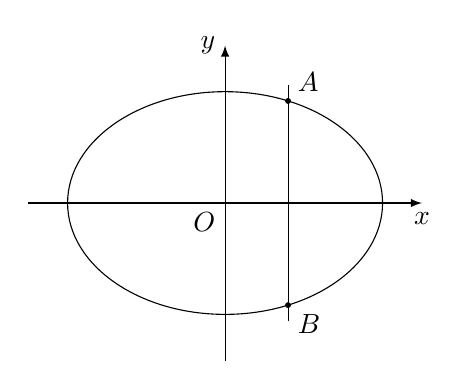
\begin{tikzpicture}[>=latex]
        \draw [->] (-2.5,0) -- (2.5,0) node [below] {$x$};
        \draw [->] (0,-2) -- (0,2) node [left] {$y$};
        \draw (0,0) node [below left] {$O$};
        \draw [name path = ellipse] (0,0) ellipse (2 and {sqrt(2)});
        \draw [name path = line] (0.8,-1.5) -- (0.8,1.5);
        \draw [name intersections = {of = line and ellipse, by = {A,B}}];
        \filldraw (A) circle (0.03) node [above right] {$A$};
        \filldraw (B) circle (0.03) node [below right] {$B$};
    \end{tikzpicture}
\end{center}
(1) 记$F_1,F_2$是椭圆$\Gamma$的左右焦点, 若直线$AB$过$F_2$, 当$M$到$F_1$的距离与到直线$AB$的距离相等时, 求点$M$的横坐标;\\
(2) 若点$M,A$关于$y$轴对称, 当$\triangle MAB$的面积最大时, 求直线$MB$的方程;\\
(3) 设直线$MA$和$MB$与$x$轴分别交于$PQ$, 证明: $|OP|\cdot |OQ|$为定值.
\item 已知无穷数列$\{a_n\}$的各项均为正数, 其前$n$项和为$S_n$, $a_1=4$.\\
(1) 如果$a_2=2$, 且对于一切正整数$n$, 均有$a_n\cdot a_{n+2}=a_{n+1}^2$, 求$S_n$;\\
(2) 如果对于一切正整数$n$, 均有$a_n\cdot a_{n+1}=S_n$, 求$S_n$;\\
(3) 如果对于一切正整数$n$, 均有$a_n+a_{n+1}=3S_n$, 证明: $a_{3n-1}$能被$8$整除.
'[]








\end{enumerate}
\end{document}